\section*{Methods}
\label{Methods}
%
The psychometric method used for stimuli presentation is not one of the classical methods but is one of the adaptive methods, namely \textit{Transformed Up/Down Method}. Instead of pre-chosen stimuli intensities the stimuli intensities are determined by previous response and thus dose not depend on a qualified guess on where the threshold might be, same goes for other adaptive methods. By using an adaptive method the efficiency is maximizes because the stimuli presentations converges upon threshold and does not present stimuli that are faraway from threshold, \parencite[p. 287]{PDF:Hearing}. There are different strategies on how to determine the needed step size e.g. it can be fixed or change as the presentations converge upon the threshold, \parencite[p. 22]{PDF:Psychoacoustic}. In this study it is decided to use a changing step size, the steps will chance in logarithmic manner so that the steps are either halved or doubled according to the previous response. Apart from higher efficiency \textit{Transformed Up/Down Method} yield higher accuracy compared to e.g. \textit{Method of Constant Stimuli} because the step size is altered according to previous response. Furthermore \textit{Transformed Up/Down Method} follow the test subject's response criterions so it always adjusts the stimuli intensities according to the answers.  

The specific up/down rules are chosen so that the stimuli intensities will converge around threshold read as close to 75 \%, on a psychometric function, as possible. To achieve this the up/down rules are defined as one-up and two-down, which will result in a threshold read at 70.7 \%, \parencite[p. 22]{PDF:Psychoacoustic}. This rule implies that one-up is a result of an incorrect answer, which will lead to an increase in stimuli intensity and two-down is a result of two in a row correct answer, which will lead to a decrease in stimuli intensity. According to \textcite[p. 293]{PDF:Hearing} the probability of an increasing stimuli intensity due to an incorrect answer is: 
%
\begin{equation}
	(1-p)+p\cdot(1-p)
\end{equation}  
%
And for a decreasing stimuli intensity due to two correct answers in a row: 
%
\begin{equation}
	p\cdot p = p^2
\end{equation}    
%       
According to \textcite[p. 293]{PDF:Hearing} the chosen strategy will converge on a point where both rules have the same probability, which is 0.5. For a decreasing stimuli intensity the probability is therefore:
%
\begin{equation}
	p^2=0.5
\end{equation}  
%
And the probability for a single correct answer is: 
%
\begin{equation}
	p = \sqrt{p^2} \Rightarrow p = \sqrt{0.5^2} = 0.707
\end{equation}
%
So the probability for a single correct answer is 70.7 \%. On \autoref{fig:IllustrationUpDown} an illustration of the psychometric function for Transformed one-up and two-down method is presented. 
%
\begin{figure}[H]
	\centering
	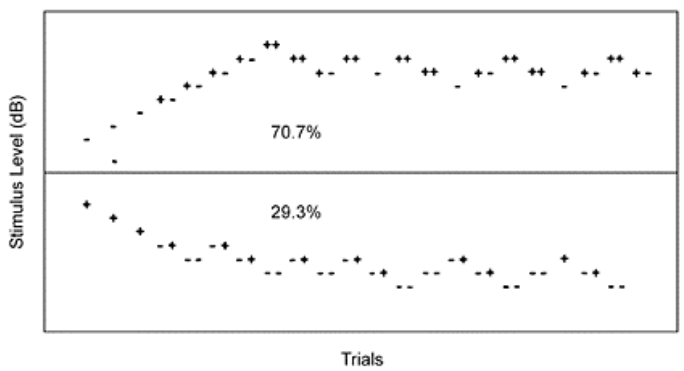
\includegraphics[resolution=300,width=0.7\textwidth]{Figure/IllustrationOfUpDown}
	\caption{An illustration of how the stimuli intensity converges upon threshold at 70.7 \% (upper frame) and 29.3 \% (lower frame), \parencite[p. 294]{PDF:Hearing}. In the upper frame the minuses indicates an incorrect response and the pluses indicate a correct response, and vice versa in the lower frame.}
	\label{fig:IllustrationUpDown}
\end{figure}
\noindent
%
The threshold is 





Diskuter metodevalg